\section{GraphTypes.h File Reference}
\label{GraphTypes_8h}\index{GraphTypes.h@{GraphTypes.h}}


\subsection{Detailed Description}
\begin{Desc}
\item[Author:]Troy Taillefer \end{Desc}


\begin{Desc}
\item[Version:]0.1 \end{Desc}
\begin{Desc}
\item[Date:]Decemeber 2, 2007 This contains the basic type of the scene grap back end representation \end{Desc}


Definition in file {\bf GraphTypes.h}.

{\tt \#include $<$boost/graph/adjacency\_\-list.hpp$>$}\par
{\tt \#include $<$boost/graph/graphviz.hpp$>$}\par


Include dependency graph for GraphTypes.h:\nopagebreak
\begin{figure}[H]
\begin{center}
\leavevmode
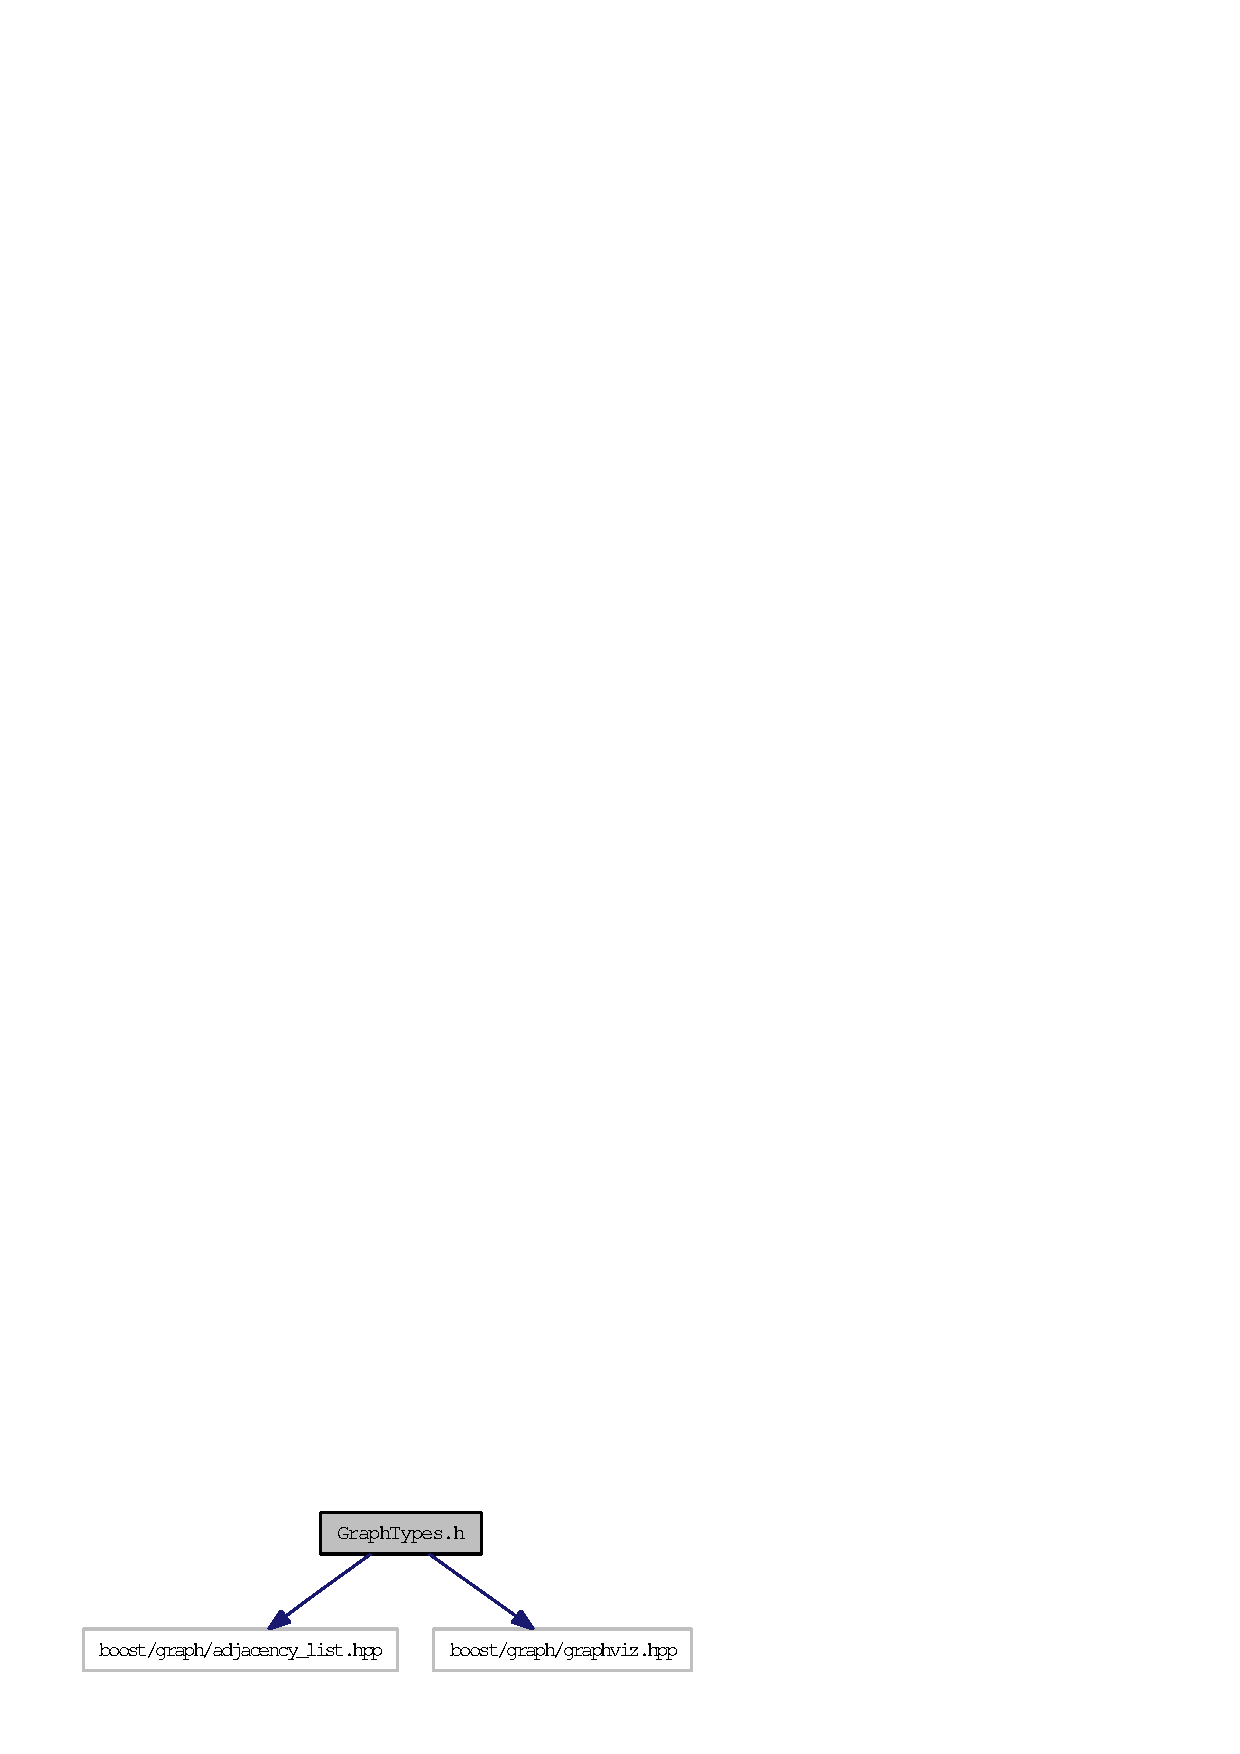
\includegraphics[width=168pt]{GraphTypes_8h__incl}
\end{center}
\end{figure}


This graph shows which files directly or indirectly include this file:\nopagebreak
\begin{figure}[H]
\begin{center}
\leavevmode
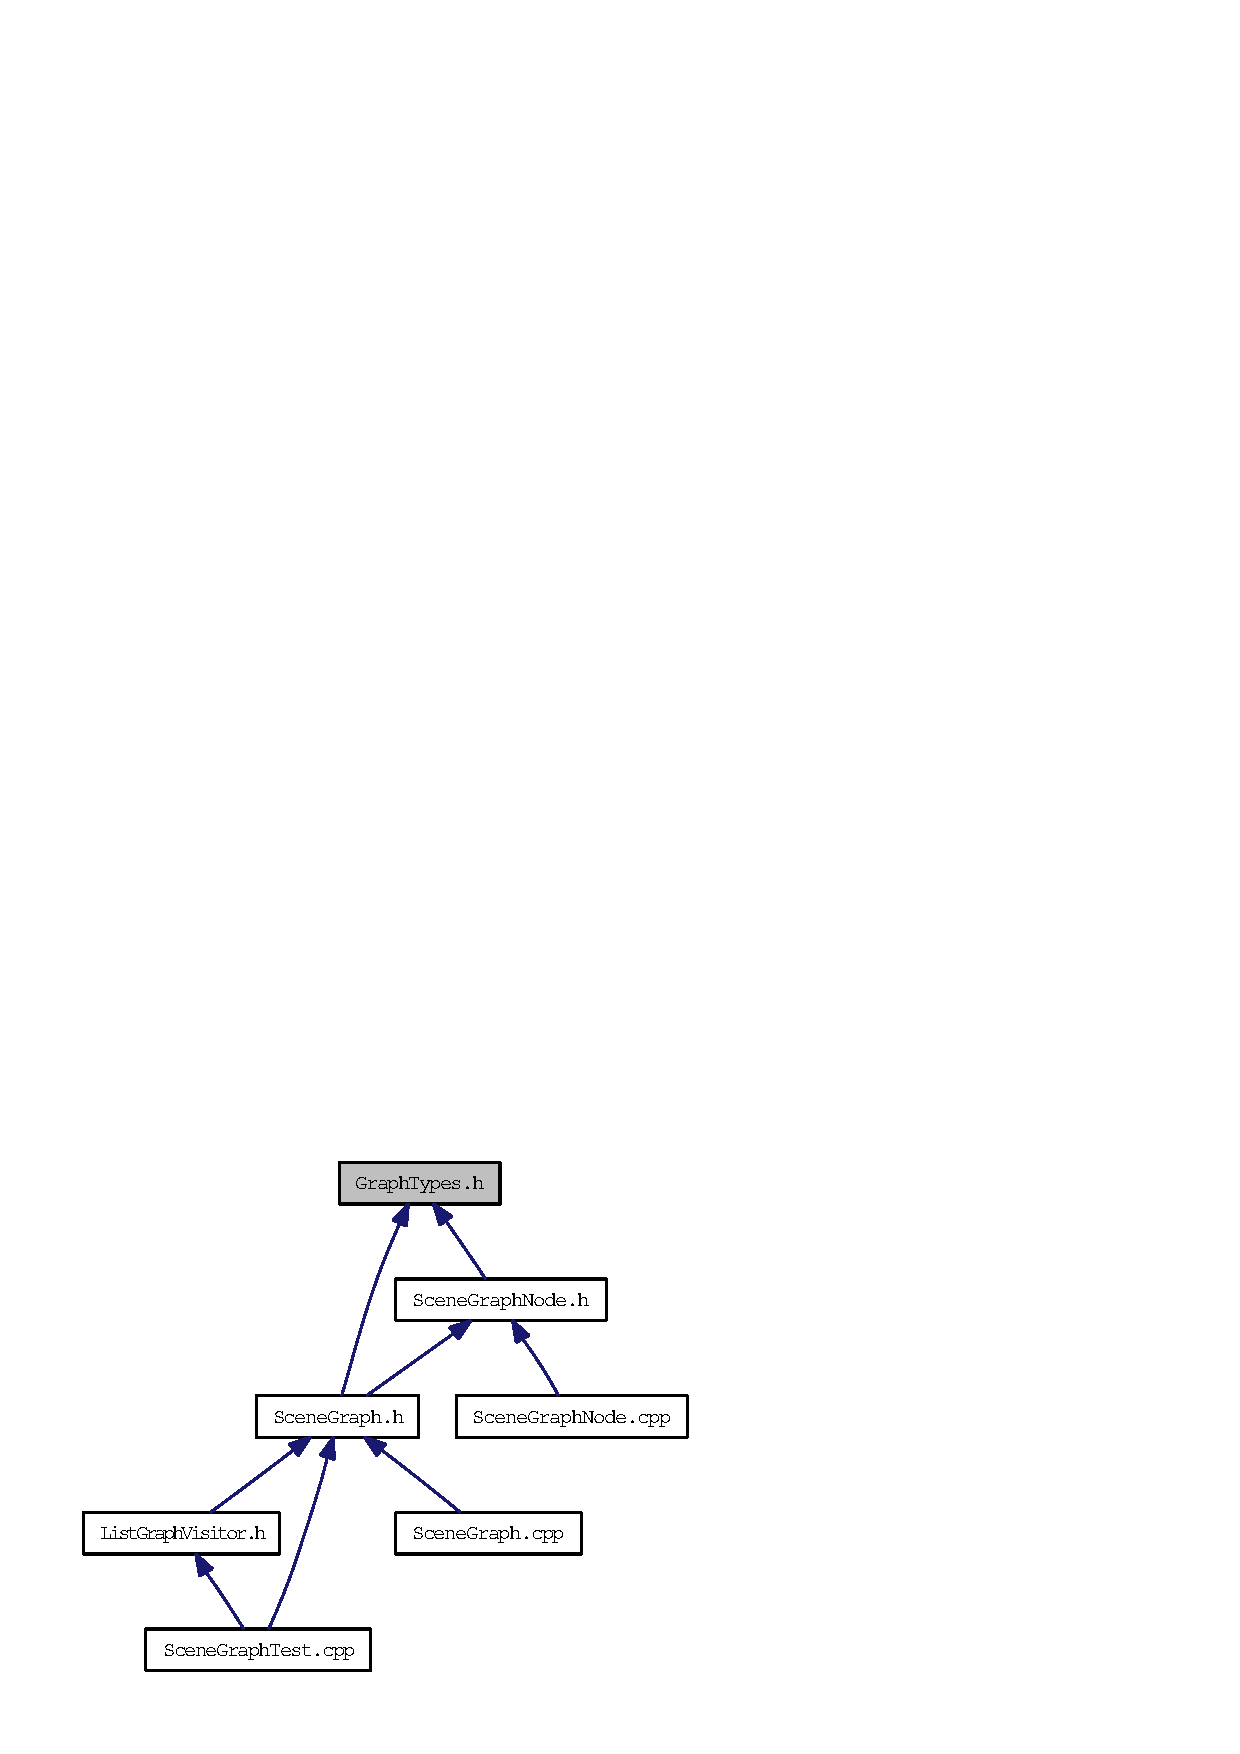
\includegraphics[width=166pt]{GraphTypes_8h__dep__incl}
\end{center}
\end{figure}
\subsection*{Typedefs}
\begin{CompactItemize}
\item 
typedef boost::adjacency\_\-list$<$ boost::vecS, boost::vecS, boost::directedS, boost::property$<$ boost::vertex\_\-name\_\-t, std::string $>$, boost::no\_\-property $>$ {\bf graph\_\-type}
\item 
typedef boost::graph\_\-traits$<$ {\bf graph\_\-type} $>$::{\bf vertex\_\-descriptor} {\bf vertex\_\-descriptor}
\end{CompactItemize}
\subsection*{Enumerations}
\begin{CompactItemize}
\item 
enum {\bf NodeType} \{ {\bf GroupNodeType}
 \}
\end{CompactItemize}
\subsection*{Functions}
\begin{CompactItemize}
\item 
std::string {\bf nodeTypeToString} ({\bf NodeType} nodeType)
\end{CompactItemize}


\subsection{Typedef Documentation}
\index{GraphTypes.h@{GraphTypes.h}!graph\_\-type@{graph\_\-type}}
\index{graph\_\-type@{graph\_\-type}!GraphTypes.h@{GraphTypes.h}}
\subsubsection{\setlength{\rightskip}{0pt plus 5cm}typedef boost::adjacency\_\-list$<$boost::vecS, boost::vecS, boost::directedS, boost::property$<$boost::vertex\_\-name\_\-t, std::string $>$, boost::no\_\-property $>$ {\bf graph\_\-type}}\label{GraphTypes_8h_dda532105e3fe044cd87d00a26f4977d}




Definition at line 13 of file GraphTypes.h.\index{GraphTypes.h@{GraphTypes.h}!vertex\_\-descriptor@{vertex\_\-descriptor}}
\index{vertex\_\-descriptor@{vertex\_\-descriptor}!GraphTypes.h@{GraphTypes.h}}
\subsubsection{\setlength{\rightskip}{0pt plus 5cm}typedef boost::graph\_\-traits$<$ {\bf graph\_\-type} $>$::{\bf vertex\_\-descriptor} {\bf vertex\_\-descriptor}}\label{GraphTypes_8h_b2dd3626f9b1623eebd5e72d7064dc37}




Definition at line 17 of file GraphTypes.h.

\subsection{Enumeration Type Documentation}
\index{GraphTypes.h@{GraphTypes.h}!NodeType@{NodeType}}
\index{NodeType@{NodeType}!GraphTypes.h@{GraphTypes.h}}
\subsubsection{\setlength{\rightskip}{0pt plus 5cm}enum {\bf NodeType}}\label{GraphTypes_8h_cac9cbaeea226ed297804c012dc12b16}


\begin{Desc}
\item[Enumerator: ]\par
\begin{description}
\index{GroupNodeType@{GroupNodeType}!GraphTypes.h@{GraphTypes.h}}\index{GraphTypes.h@{GraphTypes.h}!GroupNodeType@{GroupNodeType}}\item[{\em 
GroupNodeType\label{GraphTypes_8h_cac9cbaeea226ed297804c012dc12b16f14b754d0197656fe38f927614758139}
}]\end{description}
\end{Desc}



Definition at line 19 of file GraphTypes.h.

\subsection{Function Documentation}
\index{GraphTypes.h@{GraphTypes.h}!nodeTypeToString@{nodeTypeToString}}
\index{nodeTypeToString@{nodeTypeToString}!GraphTypes.h@{GraphTypes.h}}
\subsubsection{\setlength{\rightskip}{0pt plus 5cm}std::string nodeTypeToString ({\bf NodeType} {\em nodeType})}\label{GraphTypes_8h_0d6de0bb6213b4ac98a1e84d679902b6}




Definition at line 21 of file GraphTypes.h.

References GroupNodeType.

Referenced by SceneGraphNode::toString().

Here is the caller graph for this function:\nopagebreak
\begin{figure}[H]
\begin{center}
\leavevmode
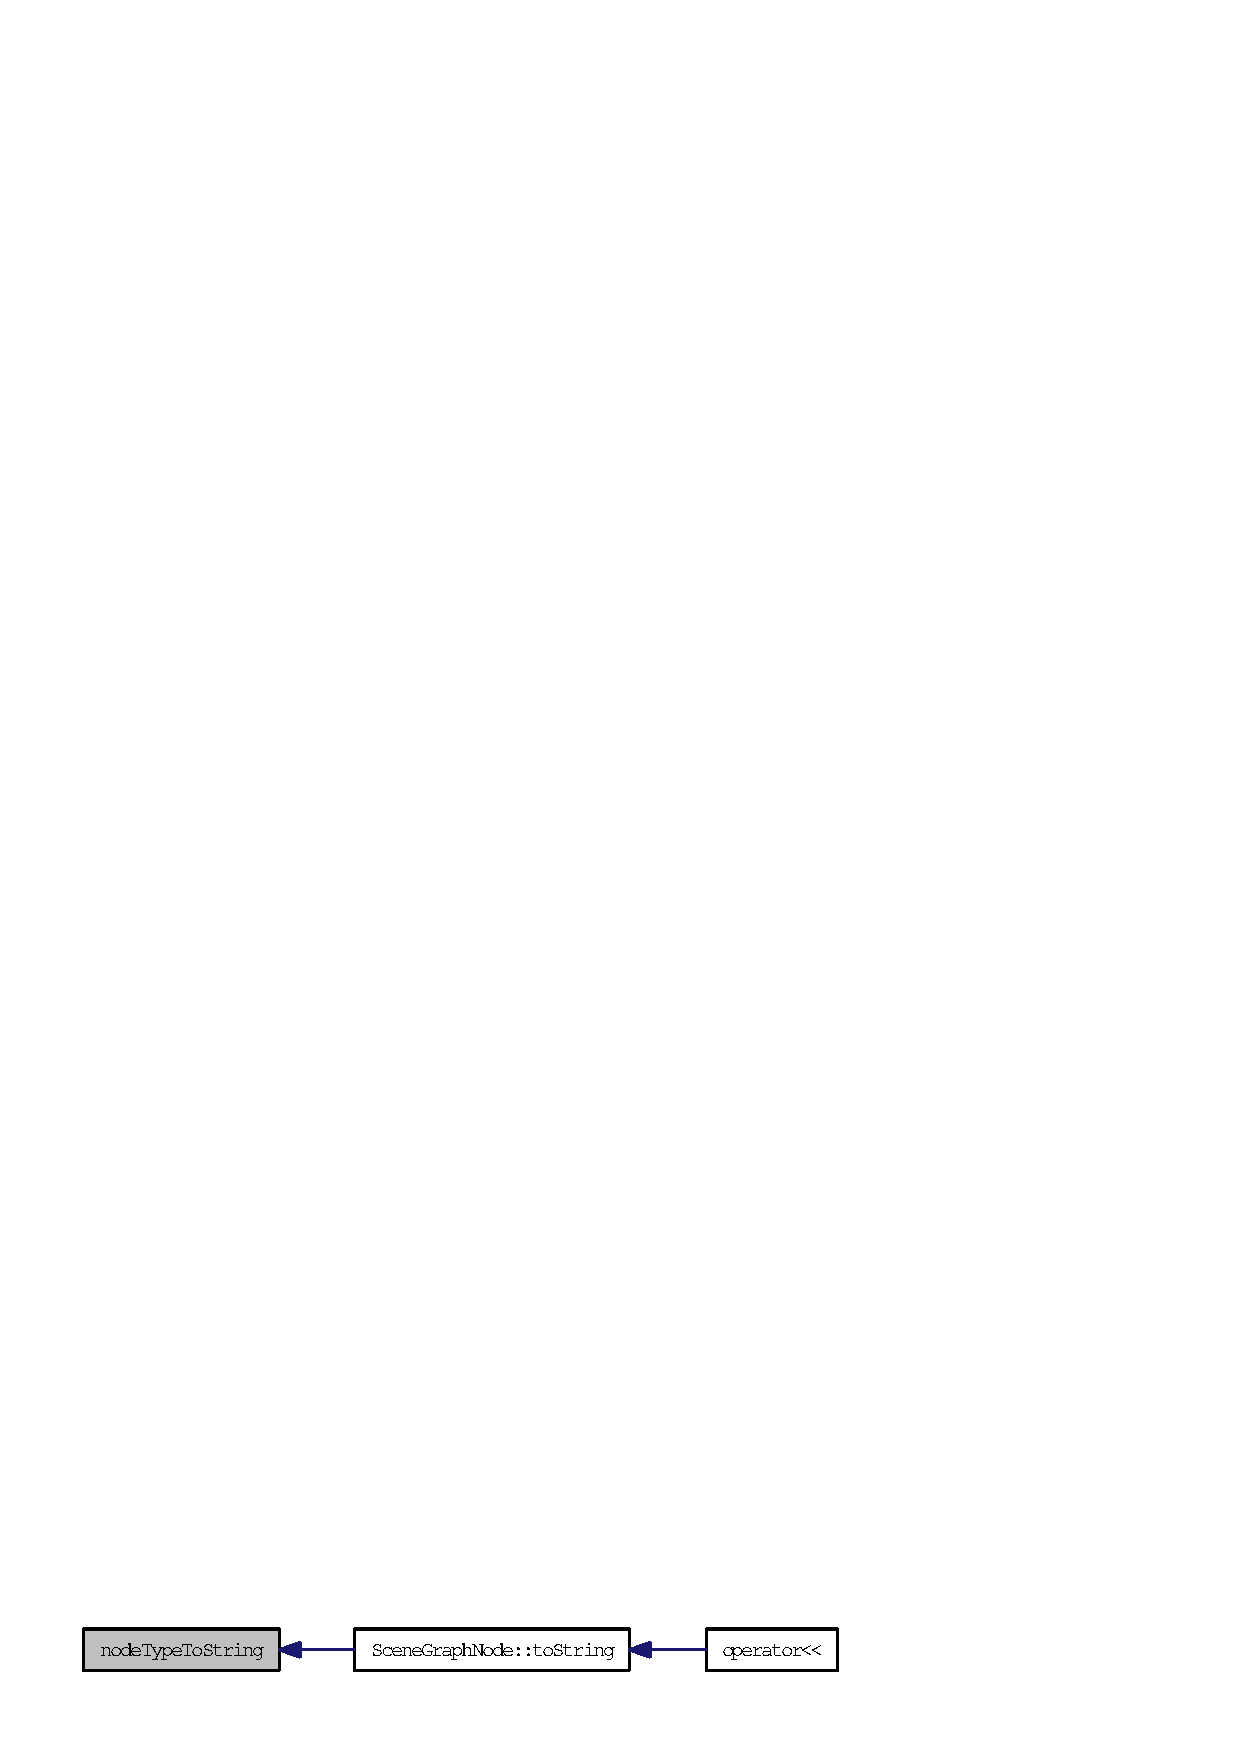
\includegraphics[width=203pt]{GraphTypes_8h_0d6de0bb6213b4ac98a1e84d679902b6_icgraph}
\end{center}
\end{figure}
